\chapter{Requisitos e modelagem do sistema}\label{cap:requisitos}

Este capítulo consolida os requisitos do S.R.I. e os artefatos de modelagem produzidos durante o estágio. São apresentados os casos de uso do sistema, a especificação detalhada do caso de uso de gerenciamento de locais, os modelos de classes, de dados e de implantação e, por fim, os requisitos funcionais e não funcionais, as premissas e as dependências do produto.

\section{Casos de uso do sistema}

O escopo funcional do S.R.I. é composto por quatro casos de uso, todos associados ao ator Usuário, que representa o motorista ou entregador que utiliza o aplicativo para planejar e executar suas rotas. O diagrama de casos de uso do sistema é apresentado na Figura \ref{fig:caso-de-uso}.

O caso de uso Gerenciar Locais responde pelo cadastro, pela consulta, pela atualização e pela exclusão dos pontos de interesse que servirão de paradas nas rotas. O caso de uso Gerar Rotas utiliza os locais previamente cadastrados para compor trajetos ponto a ponto e circuitos com retorno ao ponto inicial. O caso de uso Gerenciar Rotas Salvas registra os trajetos gerados e permite consultá-los, atualizá-los e excluí-los para reutilização em entregas futuras. O caso de uso Gerenciar Usuário realiza as operações de cadastro, autenticação e manutenção da conta do usuário \cite{sriEspecUC2026}.

\begin{figure}[!ht]
    \centering
    \caption{Diagrama de casos de uso do S.R.I.}
    \label{fig:caso-de-uso}
    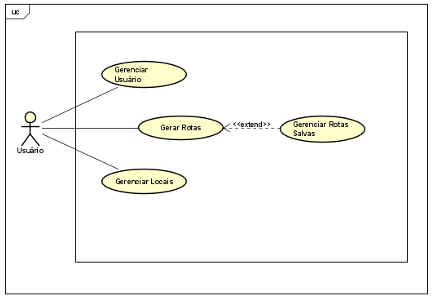
\includegraphics[width=0.8\linewidth]{imagens/caso-de-uso.png}
    \vspace{2pt}
    \footnotesize Fonte: o próprio autor (2026)
\end{figure}

\section{Especificação do caso de uso UC01: Gerenciar Locais}

O caso de uso UC01 tem como ator o Usuário e consiste na possibilidade de criar, ler, atualizar e excluir os locais que serão utilizados posteriormente na criação de rotas \cite{sriEspecUC2026}. As pré-condições estabelecem que o aplicativo deve estar aberto e que é necessária conexão à internet, uma vez que a conversão do endereço informado em coordenadas geográficas depende de serviço externo. As pós-condições preveem que um identificador de local seja gerado e que o local seja adicionado à lista exibida na tela inicial.

\subsection{Fluxo básico}

O fluxo básico descreve a sequência de eventos que deve ocorrer de forma correta para o cadastro de um novo local \cite{sriEspecUC2026}:

\begin{enumerate}
    \item o Usuário clica no botão de adição para cadastrar um novo local;
    \item o Sistema solicita as informações do local, nome e endereço;
    \item o Usuário insere as informações solicitadas e aciona a opção de salvar e buscar no mapa;
    \item o Sistema identifica se o local já existe;
    \item o Sistema adiciona o local à lista;
    \item o Usuário pode selecionar a opção de atualizar as informações do local;
    \item o Sistema valida se os campos não estão vazios e exibe um indicador de carregamento;
    \item o Sistema envia o endereço digitado para o serviço de geocodificação do OpenStreetMap (Nominatim);
    \item o Sistema recebe a latitude e a longitude correspondentes ao endereço;
    \item o Sistema salva todas as informações, nome, endereço, latitude e longitude, no banco de dados local SQLite;
    \item o Sistema fecha a tela de formulário, retorna à tela inicial e atualiza a lista, exibindo o novo ponto salvo.
\end{enumerate}

\subsection{Fluxos alternativos}

O fluxo alternativo FA01 trata da edição de um ponto existente. Na tela inicial, o Usuário aciona o ícone de edição ao lado de um ponto já salvo; o Sistema abre a tela de formulário com os dados preenchidos; o fluxo retorna ao passo 3 do fluxo básico, com a diferença de que, no passo 10, o Sistema atualiza o registro existente no banco de dados em vez de criar um novo \cite{sriEspecUC2026}.

O fluxo alternativo FA02 trata da exclusão de um ponto. Na tela inicial, o Usuário aciona o ícone de exclusão ao lado de um ponto; o Sistema remove o registro do banco de dados SQLite; e o Sistema atualiza a lista e exibe uma mensagem temporária de confirmação da exclusão \cite{sriEspecUC2026}.

O fluxo alternativo FA03 trata da visualização no mapa. Na tela inicial, o Usuário aciona o nome de um ponto salvo na lista; o Sistema abre a tela de mapa; e o Sistema renderiza o mapa centralizado na latitude e na longitude salvas, exibindo um marcador no ponto correspondente \cite{sriEspecUC2026}.

A interação entre os componentes do sistema durante o cadastro de um local é representada pelo diagrama de sequência da Figura \ref{fig:sequencia-gerenciar-locais}, que evidencia a ordem das mensagens trocadas entre a interface, a camada de persistência e o serviço de geocodificação. O ciclo de vida do local cadastrado, desde a abertura do formulário até a exclusão do registro, é representado pelo diagrama de estados da Figura \ref{fig:estado-gerenciar-locais}.

\begin{figure}[p]
    \centering
    \caption{Diagrama de sequência do caso de uso UC01}
    \label{fig:sequencia-gerenciar-locais}
    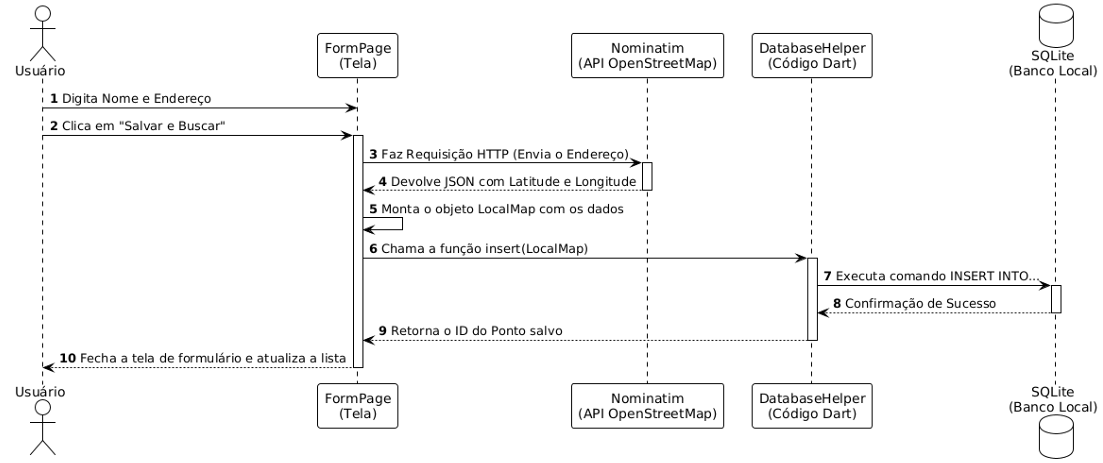
\includegraphics[angle=90,width=21cm]{imagens/sequencia-gerenciar-locais.png}
    \vspace{2pt}
    \footnotesize Fonte: o próprio autor (2026)
\end{figure}

\begin{figure}[!ht]
    \centering
    \caption{Diagrama de estados do caso de uso UC01}
    \label{fig:estado-gerenciar-locais}
    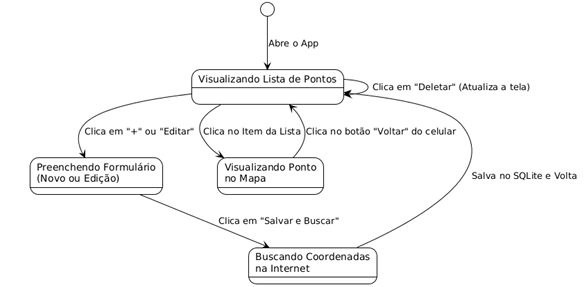
\includegraphics[width=0.8\linewidth]{imagens/estado-gerenciar-locais.png}
    \vspace{2pt}
    \footnotesize Fonte: o próprio autor (2026)
\end{figure}

\section{Demais casos de uso}

O caso de uso UC02, Gerar Rotas, tem como ator o Usuário e como pré-condição a existência de ao menos dois locais cadastrados. O fluxo principal compreende a seleção dos locais que comporão o trajeto, a escolha entre a modalidade ponto a ponto e a modalidade em circuito, o cálculo do percurso e a apresentação do resultado sobre o mapa, com a indicação da distância total e do tempo estimado de deslocamento \cite{sriEspecUC2026}.

O caso de uso UC03, Gerenciar Rotas Salvas, permite registrar um trajeto calculado para reutilização posterior e realizar as operações de consulta, atualização e exclusão sobre os registros existentes. A principal finalidade do caso de uso é eliminar a necessidade de redefinir manualmente, a cada jornada, os trajetos que se repetem com frequência na rotina do entregador \cite{sriEspecUC2026}.

O caso de uso UC04, Gerenciar Usuário, responde pelo cadastro da conta, pela autenticação e pela manutenção dos dados do usuário. O requisito de autenticação é obrigatório, de modo que não existe a possibilidade de acesso às funcionalidades do sistema sem um usuário previamente identificado \cite{sriEspecComp2025}.

\section{Modelo de classes}

O modelo de classes do sistema, apresentado na Figura \ref{fig:diagrama-de-classes}, descreve as entidades que sustentam as funcionalidades previstas e os relacionamentos existentes entre elas. A classe que representa o local cadastrado concentra os atributos de nome, endereço, latitude e longitude e mantém associação com a classe que representa a rota, uma vez que uma rota é composta por um conjunto ordenado de locais. A modelagem contempla ainda as classes responsáveis pela autenticação do usuário e pelo armazenamento das rotas salvas, cujos relacionamentos garantem que cada trajeto registrado permaneça vinculado ao usuário que o criou.

\begin{figure}[!ht]
    \centering
    \caption{Diagrama de classes do S.R.I.}
    \label{fig:diagrama-de-classes}
    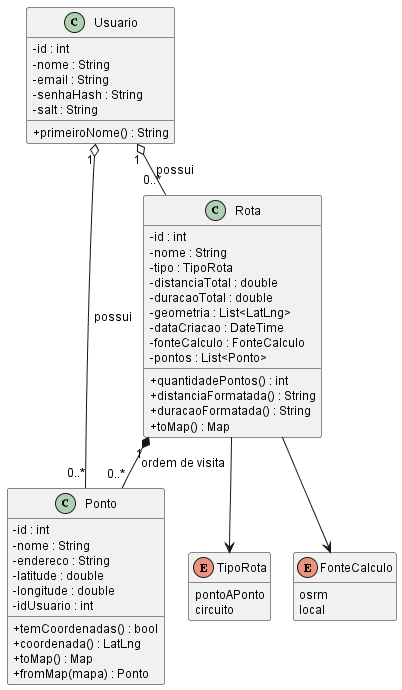
\includegraphics[width=0.56\linewidth]{imagens/diagrama-de-classes.png}
    \vspace{2pt}
    \footnotesize Fonte: o próprio autor (2026)
\end{figure}

\section{Modelo de dados}

O diagrama de entidade e relacionamento, apresentado na Figura \ref{fig:der}, representa a estrutura do banco de dados local do aplicativo. O modelo materializa as decisões do modelo de classes em tabelas, chaves primárias e relacionamentos, de modo a assegurar a integridade dos dados gravados no dispositivo.

A entidade que armazena os locais reúne o identificador do registro, o nome atribuído pelo usuário, o endereço informado e as coordenadas de latitude e longitude obtidas na geocodificação. As entidades que representam as rotas e os itens de rota permitem registrar a sequência ordenada de locais que compõe cada trajeto, preservando a ordem definida no cálculo. A entidade de usuário mantém os dados de identificação e de autenticação, e a associação entre usuário, locais e rotas garante que cada informação permaneça vinculada ao seu proprietário.

\begin{figure}[!ht]
    \centering
    \caption{Diagrama de entidade e relacionamento do S.R.I.}
    \label{fig:der}
    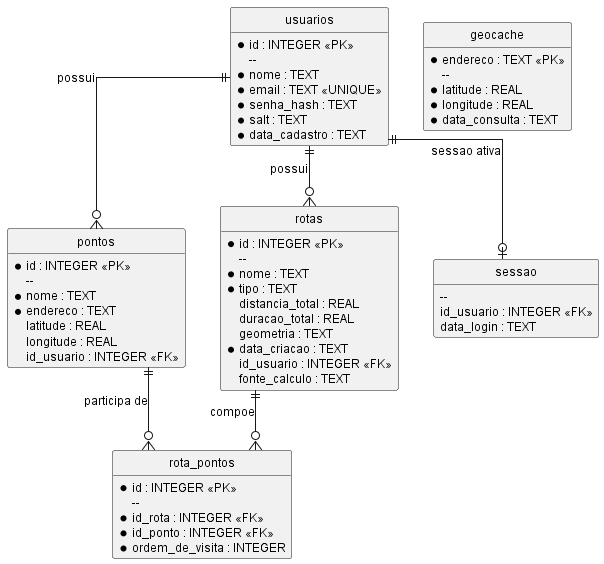
\includegraphics[width=0.8\linewidth]{imagens/der.png}
    \vspace{2pt}
    \footnotesize Fonte: o próprio autor (2026)
\end{figure}

\section{Arquitetura de implantação}

O diagrama de implantação, apresentado na Figura \ref{fig:implantacao}, descreve a distribuição dos componentes do sistema. O aplicativo é instalado no dispositivo móvel do usuário e executa de forma autônoma as funcionalidades de interface, de controle e de persistência local, apoiando-se no banco de dados SQLite embarcado. As dependências externas restringem-se aos serviços acessados pela rede: o serviço de busca e geocodificação do OpenStreetMap, responsável por converter endereços em coordenadas, o servidor de blocos cartográficos, que fornece as imagens do mapa, e o serviço de roteamento por vias, que devolve a geometria e as distâncias do trajeto calculado.

Essa distribuição de responsabilidades explica por que o cadastro de locais e a consulta aos registros permanecem funcionais mesmo em situação de conectividade intermitente, enquanto as operações de geocodificação e de cálculo de rota dependem obrigatoriamente do acesso à rede, conforme estabelecido nas premissas do produto \cite{sriVisao2025}.

\begin{figure}[!ht]
    \centering
    \caption{Diagrama de implantação do S.R.I.}
    \label{fig:implantacao}
    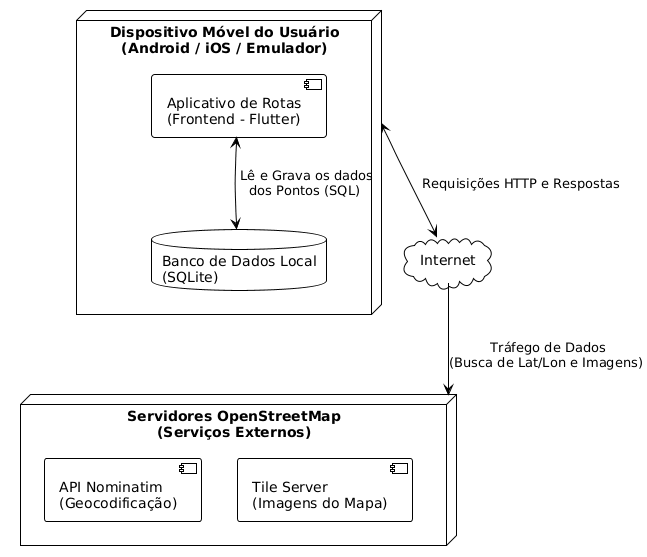
\includegraphics[width=0.8\linewidth]{imagens/implantacao.png}
    \vspace{2pt}
    \footnotesize Fonte: o próprio autor (2026)
\end{figure}

\section{Requisitos funcionais}

Os requisitos funcionais do sistema foram consolidados a partir das especificações de caso de uso e do documento de visão \cite{sriEspecUC2026, sriVisao2025}. A Tabela \ref{tab:requisitos-funcionais} apresenta os requisitos identificados e a prioridade atribuída a cada um.

\begin{table}[!ht]
    \centering
    \caption{Requisitos funcionais do S.R.I.}
    \label{tab:requisitos-funcionais}
    \begin{tabular}{p{1.4cm} p{8.6cm} p{3.4cm}}
        \hline
        \textbf{Código} & \textbf{Descrição} & \textbf{Prioridade} \\
        \hline
        RF01 & Permitir o cadastro de locais com nome, endereço e coordenadas geográficas obtidas por geocodificação. & Alta \\
        \hline
        RF02 & Permitir a consulta, a atualização e a exclusão dos locais cadastrados. & Alta \\
        \hline
        RF03 & Exibir os locais cadastrados em lista e representar cada um deles por marcador sobre o mapa. & Alta \\
        \hline
        RF04 & Gerar rotas ponto a ponto a partir da seleção de origem e destino. & Alta \\
        \hline
        RF05 & Gerar rotas em circuito, com passagem por múltiplos pontos e retorno ao ponto inicial. & Alta \\
        \hline
        RF06 & Permitir salvar as rotas geradas, bem como consultá-las, atualizá-las e excluí-las. & Média \\
        \hline
        RF07 & Permitir o cadastro e a autenticação do usuário, condicionando o acesso ao sistema à identificação prévia. & Alta \\
        \hline
        RF08 & Apresentar a distância total e o tempo estimado de deslocamento de cada rota calculada. & Média \\
        \hline
    \end{tabular}
    \vspace{2pt}
    \footnotesize Fonte: o próprio autor (2026), com base em \citeonline{sriEspecUC2026} e \citeonline{sriVisao2025}
\end{table}

\section{Requisitos não funcionais}

Os requisitos não funcionais foram extraídos da Especificação Complementar, que reúne os requisitos do sistema não capturados diretamente pelos casos de uso \cite{sriEspecComp2025}. A Tabela \ref{tab:requisitos-nao-funcionais} apresenta esses requisitos organizados por categoria.

\begin{table}[!ht]
    \centering
    \caption{Requisitos não funcionais do S.R.I.}
    \label{tab:requisitos-nao-funcionais}
    \begin{tabular}{p{3.0cm} p{10.4cm}}
        \hline
        \textbf{Categoria} & \textbf{Descrição} \\
        \hline
        Disponibilidade & O aplicativo deve estar disponível em tempo integral na sua versão mais recente, por executar de forma ativa no dispositivo móvel. \\
        \hline
        Autenticação & O acesso às funcionalidades exige usuário previamente cadastrado, não havendo possibilidade de utilização anônima. \\
        \hline
        Desempenho & O tempo para disponibilizar a resposta de uma requisição deve ser inferior a 30 segundos; requisições acima desse limite caracterizam falha de conexão entre o sistema e a fonte de dados. \\
        \hline
        Utilidade & O aplicativo opera em plataforma móvel e requer conexão de internet para o acesso aos serviços externos. \\
        \hline
        Suportabilidade & O sistema deve executar em dispositivos móveis, com hardware compatível com aplicativos de transporte, e é distribuído por meio de pacote de instalação. \\
        \hline
        Interfaces de usuário & O usuário deve realizar autenticação para acessar as funcionalidades; a interface deve ser simples e adaptada para uso em movimento. \\
        \hline
        Interfaces de hardware & O dispositivo deve dispor de acesso à internet e de receptor de GPS compatível com a operação. \\
        \hline
        Interfaces de software & A construção utiliza o framework Flutter, a linguagem Dart, o banco de dados SQLite e serviços de geolocalização, com desenvolvimento no Visual Studio Code. \\
        \hline
        Interfaces de comunicação & A comunicação entre o aplicativo e o usuário é disponibilizada integralmente pelo dispositivo móvel. \\
        \hline
        Componentes comprados & Todo o desenvolvimento foi realizado com ferramentas de código aberto; nenhum componente foi adquirido. \\
        \hline
        Licença & O sistema não exige licenças, uma vez que todos os recursos utilizados são de uso livre. \\
        \hline
        Padrões aplicáveis & A documentação e a modelagem seguem os padrões da UML e os artefatos previstos pelo processo RUP. \\
        \hline
    \end{tabular}
    \vspace{2pt}
    \footnotesize Fonte: o próprio autor (2026), com base em \citeonline{sriEspecComp2025}
\end{table}

\section{Premissas e dependências}

O documento de Visão estabelece as premissas e as dependências que condicionam a operação do sistema \cite{sriVisao2025}. Quanto às premissas, considera-se que o usuário disporá de conexão estável com a internet e de GPS ativo no dispositivo durante a utilização do aplicativo, e que o produto será compatível com as plataformas Android e iOS.

Quanto às dependências, o sistema depende de serviços externos de mapas e de geolocalização para a conversão de endereços em coordenadas e para o cálculo dos trajetos sobre a malha viária, o que vincula o comportamento das funcionalidades de rota à disponibilidade desses serviços. Estão previstas, para versões futuras, integrações com aplicativos de entrega e com sistemas de gestão logística, bem como a inclusão de recursos de visualização do tráfego em tempo real e de compartilhamento de rotas \cite{sriVisao2025}.
